\documentclass{article}
\usepackage[spanish]{babel}
\usepackage[letterpaper,top=2cm,bottom=2cm,left=3cm,right=3cm,marginparwidth=1.75cm]{geometry}


\usepackage{amsmath}
\usepackage{graphicx}
\usepackage{hyperref}
\usepackage{listings}
\lstset{language=Python}

\title{Análisis de datos con Python}
\author{Joana Guadalupe García Langarica @jg.garcialangarica}

\begin{document}
\maketitle

\section{Análisis con datos del INE}
Se obtuvo una base de datos de la página web del Instituto Nacional Electoral \cite{INE} con datos de la lista nominal de electores del país para así, con el análisis pertinente, predecir el número de casillas que se necesitarían en el estado de Guanajuato para el mes de febrero de 2021.

Usé el lenguaje de programación \textit{Python} para el manejo de información y el análisis estadístico, usando librerías como \textit{pandas} y \textit{numpy} para la realización de \textit{dataframes} y operaciones matemáticas.

\subsection{Metodología}
Las bibliotecas empleadas en este ejercicio fueron las siguientes:

\begin{lstlisting}
import numpy as np
import matplotlib.pyplot as plt
import pandas as pd 
import glob
from sklearn.linear_model import LinearRegression
\end{lstlisting}

Para empezar, leí los 16 archivos \textit{.csv} correspondientes al periodo comprendido entre septiembre del 2019 y diciembre del 2020 y los metí en en la lista \textit{allfiles}. 

\begin{lstlisting}
path = r'C:\Users\joana\Desktop\INE' # use la ruta pertinente
all_files = glob.glob(path + "/*.csv")
\end{lstlisting}

Como sólo me interesaba tener las columnas de \textsc{entidad} y \textsc{seccion} una vez en el \textit{dataframe}, inicialicé un contador que posteriormente serviría para diferenciar el primer archivo de los demás y guardar diferentes columnas.Asimismo, creé una lista para ahí guardar los \textit{dataframes} ya editados.

\begin{lstlisting}
li = []
count = 0
\end{lstlisting}

En este punto, ahora me doy cuenta que pude usar una función propia de la libreria pandas para sólo usar ciertas columnas. Sin embargo, como no sabía esto, ideé algunos \textit{ifs} dentro de un \textit{for} para sólo quedarme con las cuatro columnas que me interesaban: \textsc{entidad}, \textsc{seccion}, \textsc{lista} y/o \textsc{total\_lista}. Estas dos últimas son las columnas donde está la lista nominal total en los archivos, sin embargo como en algunos archivos es una y en otros otra, incluí ambas en el if.

\begin{lstlisting}
for filename in all_files:
    df = pd.read_csv(filename, index_col=None, thousands=',')
    
    for column in df: #eliminar aquellas columnas diferentes
        if column == 'ENTIDAD':
            pass
        elif column == 'SECCION':
            pass
        elif column == 'LISTA':
            pass
        elif column == 'TOTAL_LISTA':
            pass
        else:
            df= df.drop([column], axis=1)
        
    df = df[df.ENTIDAD == 11]
    
    if count != 0:
        for column in df: 
            if column == 'LISTA':
                pass
            elif column == 'TOTAL_LISTA':
                pass
            else:
                df= df.drop([column], axis=1)
    count = 1
    df= df.drop(df.index[3142:])
    df.reset_index(drop=True, inplace=True)
    li.append(df)
\end{lstlisting}
    
Aún discutiendo el segmento de código anterior, hice un ciclo for para que se leyeran todos los archivos en la lista \textit{all\_files}, los otros dos ciclos fueron para eliminar todas las columnas menos las que me interesaban. Incluí una línea para sólo guardar las filas que tuvieran el 11 (entidad correspondiente a Guanajuato) en la columna \textsc{entidad}. En las últimas tres líneas lo que hice fue desechar, en los archivos que lo ameritaba, todas las filas mas allá de la 3142, ya que no todos los meses tenían la misma cantidad de secciones por alguna razón, y era necesario que fuera así para hacer la regresión lineal.

Todos los \textit{dataframes} ya con las únicas 4 columnas necesarias y la entidad 11 se guardan en la lista li. Para finalizar la parte del código donde se modifica el \textit{dataframe}, concatené los 16 archivos en df, a manera de que se añadiera cada mes como una nueva columna; eliminé la primera fila del \textit{dataframe} ya concatenado pues es la sección  0, correspondiente a los extranjeros y que puede despreciarse.

\begin{lstlisting}
df = pd.concat(li, axis=1)
df = df.drop(df.index[0])
\end{lstlisting}

Guardé el \textit{dataframe} df como un arreglo de NumPy para poder hacer la regresión lineal. Definí mi x como un arreglo de NumPy del 1 al 16 (los meses del periodo estudiado), definí la función de LinearRegression como regresión\_lineal y definí una lista para almacenar las predicciones.

\begin{lstlisting}
data = np.array(df)
x = np.array([1,2,3,4,5,6,7,8,9,10,11,12,13,14,15,16])
regresion_lineal = LinearRegression()
predicciones = []
\end{lstlisting}

Inicié un ciclo \textit{for} que hiciera tantas iteraciones como la longitud de mi arreglo, esto para definir mi $y$ \textit{data}. Posteriormente usé la función para realizar la regresión lineal, remodelando x, y para que fueran de la misma dimensión.

\begin{lstlisting}
for i in range (len(data)):

    y = data[i, 3:].reshape(-1,1)
    regresion_lineal.fit(x.reshape(-1,1), y) 
    nuevo_x = np.array([18]) 
    predicciones.append(math.ceil(float(regresion_lineal.predict(nuevo_x.reshape(-1,1)))))
 \end{lstlisting}
 
 Definí una lista para guardar la cantidad de casillas a necesitar y guardé la cantidad de casillas en cada predicción con \textit{append}, dividiendo la predicción de cada sección para el mes de febrero del 2021 entre las 750 personas que votan por casilla.
 
 \begin{lstlisting}
casillas = []

for prediccion in predicciones:
    casillas.append(math.ceil(prediccion/750))
\end{lstlisting}
Usé la función de suma para conseguir el total de casillas a instalar en el 2021
\begin{lstlisting}
print(sum(casillas))
\end{lstlisting}

\subsection{Resultados}\label{res_1}
La suma de las casillas por sección arroja 7543 casillas para el estado de Guanajuato en el mes de febrero del año 2021.

\subsection{Conclusiones}
 Ya que la lista nominal por casillas es un dato más directo, comparado a la lista nominal por municipio (que por lo mismo decidí no calcular), puedo asegurar que el dato más confiable es calculado con las secciones. Pero, ¿por qué considero este dato más certero que el municipal? Pues el dato municipal es realmente un promedio, por lo que usarlo nos significa una desviación estándar mayor; por su parte, las secciones son datos más simples, no son cálculos, por lo que su desviación es mínima y, en términos estadísticos, son más confiables.
 
\section{Análisis con otra base de datos}
Para la segunda parte del proyecto, elegí una base de datos de la página web \textit{Kaggel}, llamada "Women in Movies´´ \cite{Bed} que tiene un registro de las películas albergadas en el \href{https://bechdeltest.com}{sitio web} del test de Bechdel, desde 1970 hasta el 2013. Los datos se abstrajeron del sitio en el año 2014.

El \textbf{test de Bechdel} es una regla arbitraria creada por la dibujante Alison Bechdel. Desde su origen en el '85, ha pasado de ser una broma ligera a una verdadera medida para medir la representación de las mujeres en películas y demás obras de ficción. El test consiste en tres condiciones, si una película cumple todas es considerado que pasó el test:

\begin{enumerate}
    \item Tener por lo menos dos mujeres [nombradas en el filme] que
    \item Hablen entre ellas
    \item De algo más que un hombre
\end{enumerate}

Me propuse lograr dos cosas con esta base de datos:
\begin{itemize}
    \item Predecir el número de películas que pasaron el test en el 2015 y compararlas al número real, calculado con la información propia de la página del test.
    \item Determinar cuál regla se cumple menos entre las películas de la base de datos.
\end{itemize}

\subsection{Metodología}
Las librerias empleadas en este ejercicio fueron las siguientes:

\begin{lstlisting}
import pandas as pd
import numpy as np
from typing import Set, Any 
import matplotlib.pyplot as plt
from sklearn.linear_model import LinearRegression
\end{lstlisting}

Para empezar, leí el archivo \textit{movies.csv} correspondiente a la base de datos. Navegando por internet, de nuevo sin el conocimiento de la función especial de \textit{pandas} para escoger columnas específicas, encontré una función que hace lo mismo. La usé para sólo usar las columnas correspondientes a \textit{year}, \textit{clean\_test} y \textit{binary}, que son las necesarias para contestar las cuestiones establecidas al inicio. Además, la última línea es para eliminar las opción dubious en \textit{clean\_test}, ya que no era relevante para el análisis.

\begin{lstlisting}
df = pd.read_csv("movies.csv")

    
def remove_others(df: pd, columns: Set[Any]):
    cols_total: Set[Any] = set(df.columns)
    diff: Set[Any] = cols_total - columns
    df.drop(diff, axis=1, inplace=True)
    
remove_others(df, {"year", "clean_test", "binary"})

df = df[df.clean_test != "dubious"]
\end{lstlisting}

Estas columnas son necesarias por lo siguiente
\begin{itemize}
    \item \textit{year} indica el año en el que se publicó la película. Como las regresiones se harán por año es importante.
    \item\textit{clean\_test} es un atributo que determina cuál regla no cumplió la película, o en su caso si todas se cumplieron.
    \item\textit{binary} determina si la película pasó o no el test.
\end{itemize}
Posteriormente, inicialicé una variable que serviría como condición para el \textit{for} siguiente. Observamos que toma la columna \textit{year} y define que n va en un rango de 0 al $m-10$ número de filas, esto para no tomar en cuenta las películas de 1970 a 1979. Tomé esta decisión ya que las películas de los años 70's registradas en la página eran muy pocas, y temía que alteraran de alguna manera los datos por salirse demasiado de la mediana.

\begin{lstlisting}
n = (pd.unique(df['year']))
n = n[0:-10]
\end{lstlisting}

A este punto empecé la parte del código que me ayudaría a determinar tanto la predicción, como cuál regla del test se cumplió menos. Es importante saber algunas variables usadas:

\begin{itemize}
    \item \textit{nt} es no\_talk para las películas donde hay por lo menos dos mujeres pero no hablan entre ellas.
    \item \textit{ok} para las películas que cumplen todas las reglas.
    \item \textit{nw} es no\_women para las películas donde no hay por lo menos dos mujeres.
    \item \textit{men} para las películas donde hay por lo menos dos mujeres que hablan entre sí, pero su conversación se trata de un hombre.
\end{itemize}

Definí una lista llamada dfs donde se guarda cada \textit{dataframe} correspondiente a cada año, determinado por el primer ciclo \textit{for} visible. Posteriormente definí un arreglo de \textit{NumPy} llamado ratios, para almacenar la proporción de aprobación del test respecto al total de películas.

\begin{lstlisting}
dfs = []
for i in n:
    df1 = df[df['year'] == i]
    dfs.append(df1)

ratios = []
count = 0
count_nt = 0
count_ok = 0
count_nw = 0
count_men = 0

\end{lstlisting}

Posteriormente realicé un ciclo \textit{for} para contar las películas que pasaron el test, usando la variable \textit{binary} definida anteriormente. 

\begin{lstlisting}
for df in dfs:
    for i in (df['binary']):
        if i ==  'PASS':
            count += 1
\end{lstlisting}

También definí una variable llamada \textit{ratio} que me servirá para saber, con el contador \textit{count} definido con los demás contadores, el ratio de películas que pasaron respecto al número total de películas. Esto se guardará en el arreglo \textit{ratios}.

\begin{lstlisting}        
    ratio = count/len(df['binary'])
    ratios.append(ratio)
\end{lstlisting}    
Redefiní el contador a 0 para eliminar basura y empecé un \textit{for} con condicionales \textit{if} para contar la cantidad de películas que incumplían cada regla definida anteriormente. 
\begin{lstlisting}
    count = 0
    for j in (df['clean_test']):
        if j == 'notalk':
            count_nt += 1
    
        if j == 'ok':
            count_ok += 1
    
        if j == 'nowomen':
            count_nw += 1
            
        if j == 'men':
            count_men += 1
\end{lstlisting}

Ya con esta información, decidí hacer un gráfico de pastel. Afortunadamente la librería matplotlib.pyplot tiene una función que automáticamente saca los porcentajes del grupo de datos que pongas, por lo que sólo tuve que poner en \textit{sizes} la cantidad de películas guardada en los contadores de cada regla no cumplida. El gráfico está ilustrado en la figura \ref{fig:pastel} de la sección \ref{res}.

\begin{lstlisting}
labels = 'ok', 'notalk',  'nowomen', 'men'
sizes = [count_ok, count_nt, count_nw, count_men]
colors = ['#F16A70','#B1D877','#8CDCDA','#4D4D4D']
explode = (0.1, 0, 0, 0)  

fig1, ax1 = plt.subplots()
ax1.pie(sizes, colors=colors, explode=explode,
labels=labels, autopct='%1.1f%%', shadow=False, startangle=90)
ax1.axis('equal')  

plt.savefig("reglas_pastel.png")
\end{lstlisting}

Ya para finalizar, empecé el procedimiento para la regresión lineal que me ayudaría con la predicción. Primero redefiní \textit{ratio} y \textit{n} para que fueran arreglos \textit{NumPy} para poder hacer la regresión. Después, usando la función LinearRegression importada desde el inició, realicé la regresión lineal así como la predicción para el 2015. Tanto la predicción exclusiva del año, como Y\_pred necesaria para modelarla en la gráfica. Así, obtuve la gráfica ilustrada en la figura \ref{fig:pred} de la sección \ref{res}.

Finalmente imprimí la predicción para el año 2015, usando el modelo de predicción ya mencionado y multiplicándolo por 100 para que arrojara un porcentaje.

\begin{lstlisting}
ratios = np.array(ratios)
n = np.array(n)

model = LinearRegression().fit(n.reshape(-1,1), ratios)
pred_2015 = np.array([2015]) 
prediccion = model.predict(pred_2015.reshape(-1,1))
Y_pred = model.predict(n.reshape(-1,1))

plt.scatter(n, ratios)
plt.plot(n, Y_pred, color='red')
plt.xlabel('Años', fontsize=14)
plt.ylabel('Ratios', fontsize=14)

plt.savefig("prediccion.png")
plt.show()

print("La prediccion para el 2015 es:",
round(float(prediccion*100), 2),"%")
\end{lstlisting}

Para poder hacer la comparación de la predicción respecto a un dato real, obtuve unos datos estadísticos de la página web del sitio \cite{pag} y calculé con ellos el porcentaje de películas que pasaron el test en el 2015.

\subsection{Resultados}\label{res}

\subsubsection{La predicción}

Un total de 318 películas del 2015 se han registrado en el sitio, 199 de las cuales pasaron el test de Bechdel. Si hacemos una regla de 3 simple obtenemos el porcentaje de películas que pasaron el test.

\begin{equation*}
    \frac{(199)(100)}{318} = \textbf{62.58\%}
\end{equation*}

La predicción calculada con el modelo de predicción fue que: en el año 2015 el \textbf{58.77\%} de las películas pasarían el test de Bechdel.

Si comparamos ambos números podemos ver que la predicción se quedó corta respecto al número real, con una diferencia que estadísticamente sí es significativa.

\begin{figure}[h!]
\centering
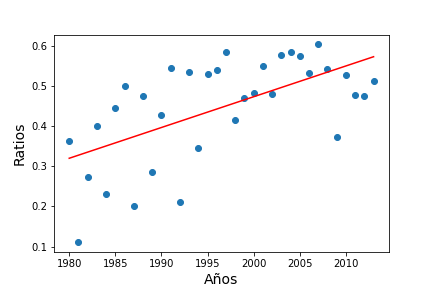
\includegraphics[scale=0.7]{prediccion.png}
\caption{\label{fig:pred}Regresión lineal de las películas que pasan el test.}
\end{figure}
\subsubsection{La regla que menos se cumplió}

Podemos observar en la figura \ref{fig:pastel} la proporción de incumplimiento de cada regla. Por simple inspección notamos que la regla \textit{ok} se cumplió más que las otras. Sin embargo, como esta variable determina que se cumplieron todas las reglas, seguimos al porcentaje más alto siguiente.

\begin{figure}[h!]
\centering
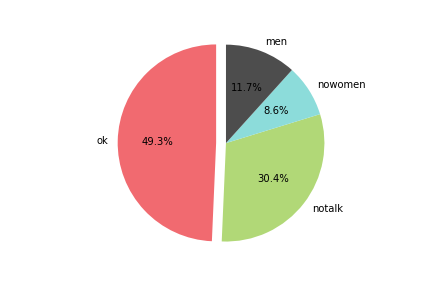
\includegraphics[scale=0.8]{reglas_pastel.png}
\caption{\label{fig:pastel}Gráfico de pastel correspondiente al incumplimiento de las reglas del test en las películas estudiadas.}
\end{figure}

Así, la regla \textit{notalk} correspondiente a las películas que tienen dos mujeres que no hablan entre ellas, resulta la regla más incumplida en las películas (1980-2013) registradas en el sitio web del test al año 2014. Del gráfico también podemos abstraer que en el 61.0\% de las películas estudiadas existen personajes mujeres que hablan entre sí, con una relativamente pequeña parte de estas conversaciones siendo exclusivamente acerca de hombres.

\subsection{Conclusiones}
El porcentaje real calculado es mayor al porcentaje predecido con el código. Este hecho puede significar muchas cosas, de la que yo estaba convencida es que el crecimiento de las películas que pasan el test a través de los años no es lineal, eso significa que el crecimiento puede tener un comportamiento exponencial.
Sin embargo, al observar la gráfica es muy sencillo notar que los puntos no se ajustan exponencialmente, por lo que es otra clase de crecimiento.

Sea cual sea, es correcto afirmar que el crecimiento real es mayor. Esto, desde un punto de vista más sociocultural, puede deberse a que en los últimos años los movimientos sociales que se encargan de luchar por la justa representación y liberación de las mujeres (como los feminismos) han tenido gran auge y mayor influencia en los medios. 

Por otro lado, la visualización del porcentaje de reglas no cumplidas arroja datos importantes para reflexionar respecto al papel que juegan las mujeres en las películas desde siempre. Observamos una pequeña cantidad (8.6\%) de películas sin mujeres en la trama, esto puede ser una buena señal respecto a la inclusión femenina en las películas: pocos directores se atreven a no incluirlas. Sin embargo, observando el 30.4\% de películas donde hay mujeres que no hablan, me llega un cuestionamiento simple: ¿será que es importante tener mujeres en el filme para llenar ciertas expectativas femeninas de los consumidores, sin llegar al punto de otorgar papeles importantes? Porque una película donde hay mujeres, pero estas no hablan o hablan exclusivamente con hombres, puede indicar una película donde no hay intención de darle importancia a esas mujeres. Además, es decepcionante que el 11.7\% de películas donde las mujeres si hablan, sólo hablan de hombres.

Para finalizar, no creo que un \textbf{49.3\%} de aprobación del test en la enorme cantidad de películas obtenidas de la base de datos sea, ni de cerca, una victoria para estos movimientos. No perdamos de vista que si el test fuese reglamentado con el género opuesto, la aplastante mayoría de las películas aquí estudiadas pasarían sin ningún problema.


\begin{thebibliography}{}

\bibitem{INE} G. Rojas Peña, \textit{Estadística de Padrón Electoral y Lista Nominal de Electores}, México: Instituto Nacional Electoral, 2020. Consultado en: 6 de Junio, 2021. [En línea]. Disponible en: \url{https://portal.ine.mx/transparencia/datos-abiertos/#/archivo/estadistica-padron-electoral-lista-nominal-electores} 

\bibitem{Bed} M. Aché, \textit{Women in Movies}, Francia: Kaggle, 2021. Consultado en: 12 de junio, 2021. [En línea]. Disponible en: \url{https://www.kaggle.com/mathurinache/women-in-movies} 
\bibitem{pag} Bechdel Test Movie List (2019). [En línea]. Disponible en: \url{https://bechdeltest.com/statistics/} 

\end{thebibliography}
\end{document}
